\documentclass[11pt,a4paper]{article}
\usepackage[left=2.5cm,right=2cm, bottom=2cm]{geometry}
\usepackage[utf8]{inputenc}
\usepackage{amsmath}
\usepackage{amsfonts}
\usepackage{amssymb}
\usepackage{amsfonts}
\usepackage{amsmath}
\usepackage{graphicx}
\usepackage{subfigure}
\usepackage{color}
\usepackage{abstract}
\usepackage{float}
\usepackage[toc,page]{appendix}
\usepackage{hyperref}
\usepackage{fancyhdr}
\usepackage{algorithm} 
\usepackage{algpseudocode} 
\usepackage{listings}
\usepackage{xcolor} % for setting colors
% set the default code style
\lstset{
	frame=tb, % draw a frame at the top and bottom of the code block
	tabsize=4, % tab space width
	showstringspaces=false, % don't mark spaces in strings
	numbers=left, % display line numbers on the left
	commentstyle=\color{green}, % comment color
	keywordstyle=\color{blue}, % keyword color
	stringstyle=\color{red} % string color
}

\pagestyle{fancy}
\fancyhf{}
\rhead{\today}
\lhead{\bfseries Alexander Leitner 01525882}
\rfoot{}



\begin{document}
\begin{center}
	\fontsize{24pt}{10pt}\selectfont
	\textsc{\textbf{Computational Science on Many-Core Architectures  Exercise 6}}
\end{center}
\section*{Example 1 Dot Product with Warp Shuffels (4 Points)}
First I want to test my implementation with a small test for a small vector.
\begin{center}
	
	\begin{minipage}[t]{0.40\textwidth}
		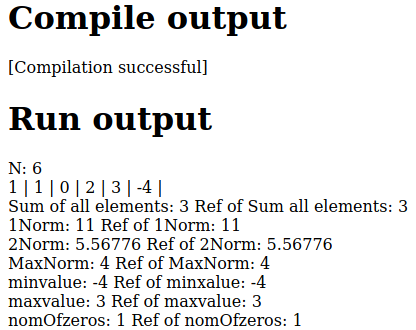
\includegraphics[width=\textwidth]{Bilder/Ex6_1}
	\end{minipage}
	
\end{center}
\subsection*{a)}
\begin{lstlisting}[language=C++, caption={additional atomicMax}]
__device__ void atomicMax(double* address, double val)
{    
	unsigned long long int* address_as_ull = (unsigned long long int*) address; 
	unsigned long long int old = *address_as_ull, assumed;
	do  
	{
		assumed = old;
		old = atomicCAS(address_as_ull, assumed, 
		__double_as_longlong(fmax(val, __longlong_as_double(assumed))));
		// atomicCAS returns the value that is stored in address AFTER the CAS
		// atomicCAS(a, b, c) --> return c
		//
	} while (assumed != old);
}
\end{lstlisting}
\begin{lstlisting}[language=C++, caption={additional atomicMin}]
 __device__ void atomicMin(double* address, double val)
{    
	unsigned long long int* address_as_ull = (unsigned long long int*) address; 
	unsigned long long int old = *address_as_ull, assumed;
	do  
	{
		assumed = old;
		old = atomicCAS(address_as_ull, assumed,
		 __double_as_longlong(fmin(val, __longlong_as_double(assumed))));
		// atomicCAS returns the value that is stored in address AFTER the CAS
		// atomicCAS(a, b, c) --> return c
		//
	} while (assumed != old);
}
\end{lstlisting}

\begin{lstlisting}[language=C++, caption={kernel for the seven operations}]
__global__ void mmsszz(double *x, double *dot, int N)
{
	__shared__ double sumofallelements[BLOCK_SIZE];
	__shared__ double einsnorm[BLOCK_SIZE];
	__shared__ double zweisnorm[BLOCK_SIZE];
	__shared__ double maxnorm[BLOCK_SIZE];
	__shared__ double maxval[BLOCK_SIZE];
	__shared__ double minval[BLOCK_SIZE];
	__shared__ double zeros[BLOCK_SIZE];
	
	if (blockDim.x * blockIdx.x < N)
	{
	unsigned int ind = threadIdx.x + blockDim.x*blockIdx.x;
	unsigned int str = blockDim.x*gridDim.x;
	double sum = 0;
	double einssum = 0;
	double zweissum = 0;
	double max = x[0];
	double min = max;
	double count = 0;
	while(ind < N)
	{
		for (int i = 0; i < N; i += str) 
		{
			sum += x[i]; // sum of all entries
			einssum += std::abs(x[i]);  // 1-norm
			zweissum += x[i] * x[i];  // 2-norm
			max = fmax(x[i], max);  // max_value
			min = fmin(x[i], min);  // min_value
			if (x[i] == 0)  // counts the zero entries
			{
				count = count + 1;
			}
		}
	ind += str;
	}
	sumofallelements[threadIdx.x] = sum;
	einsnorm[threadIdx.x] = einssum;
	zweisnorm[threadIdx.x] = zweissum;
	maxnorm[threadIdx.x] = fmax(std::abs(min), max);
	maxval[threadIdx.x] = max;
	minval[threadIdx.x] = min;
	zeros[threadIdx.x] = count;
	__syncthreads();
	for(int i = blockDim.x/2; i>0; i/=2)
	{
	__syncthreads();
	 if(threadIdx.x < i)
	 {
       sumofallelements[threadIdx.x] += sumofallelements[threadIdx.x + i];
       einsnorm[threadIdx.x] += einsnorm[threadIdx.x + i];
       zweisnorm[threadIdx.x] += zweisnorm[threadIdx.x + i];
       maxnorm[threadIdx.x] = fmax(maxnorm[threadIdx.x + i],maxnorm[threadIdx.x]);
       minval[threadIdx.x] = fmin(minval[threadIdx.x + i],minval[threadIdx.x]); 
       maxval[threadIdx.x] = fmax(maxval[threadIdx.x + i],maxval[threadIdx.x]); 
       zeros[threadIdx.x] += zeros[threadIdx.x + i];
	 }
	}
		if(threadIdx.x == 0)
		{
			atomicAdd(dot + 0,sumofallelements[0]);
			atomicAdd(dot + 1,einsnorm[0]);
			atomicAdd(dot + 2,std::sqrt(zweisnorm[0]));
			atomicMax(dot + 3, maxnorm[0]);
			atomicMin(dot + 4, minval[0]);
			atomicMax(dot + 5, maxval[0]);
			atomicAdd(dot + 6, zeros[0]);
		}
	}
}
\end{lstlisting}
\subsection*{b)}
\begin{lstlisting}[language=C++, caption={kernel for warp shuffeld}]
__global__ void analyze_x_warp(double *x, double *results, int N) 
{
	if (blockDim.x * blockIdx.x < N) 
	{
		int tid = threadIdx.x + blockDim.x * blockIdx.x; // global tid
		const int stride = blockDim.x * gridDim.x;
	
		double sum = 0.0, abs_sum = 0.0, sqr_sum = 0.0;
		// double mod_max = 0.0;
		double max = x[0];
		double min = max;
		int z_entries = 0;
		for (; tid < N; tid += stride) 
		{
			double value = x[tid];
			sum += value;
			abs_sum += std::abs(value);
			sqr_sum += value*value;
			
			min = fmin(value, min); 
			max = fmax(value, max);
			z_entries += (value)? 0 : 1;
		}
		tid = threadIdx.x; // block tid 
		double mod_max = fmax(std::abs(min), max);

		__syncthreads();
		for (int i = warpSize / 2; i != 0; i /= 2) 
		{
			//__syncthreads();
			sum += __shfl_down_sync(0xffffffff, sum, i);
			abs_sum += __shfl_down_sync(0xffffffff, abs_sum, i);
			sqr_sum += __shfl_down_sync(0xffffffff, sqr_sum, i);
			
			double tmp = __shfl_down_sync(0xffffffff, mod_max, i);
			mod_max = fmax(tmp, mod_max);
			tmp = __shfl_down_sync(0xffffffff, min, i);
			min = fmin(tmp, min);
			tmp = __shfl_down_sync(0xffffffff, max, i);
			max = fmax(tmp, max) ;
			
			z_entries += __shfl_down_sync(0xffffffff, z_entries, i);
		}  
		if (tid % warpSize == 0) // a block can consist of multiple warps
		{
			atomicAdd(results, sum);
			atomicAdd(results+1, abs_sum);
			atomicAdd(results+2, sqr_sum);
			
			atomicMax(results+3, mod_max);
			atomicMin(results+4, min);
			atomicMax(results+5, max);
			
			atomicAdd(results+6, z_entries);
		}
	}
}
\end{lstlisting}
\subsection*{c)}
\begin{center}
	
	\begin{minipage}[t]{0.49\textwidth}
		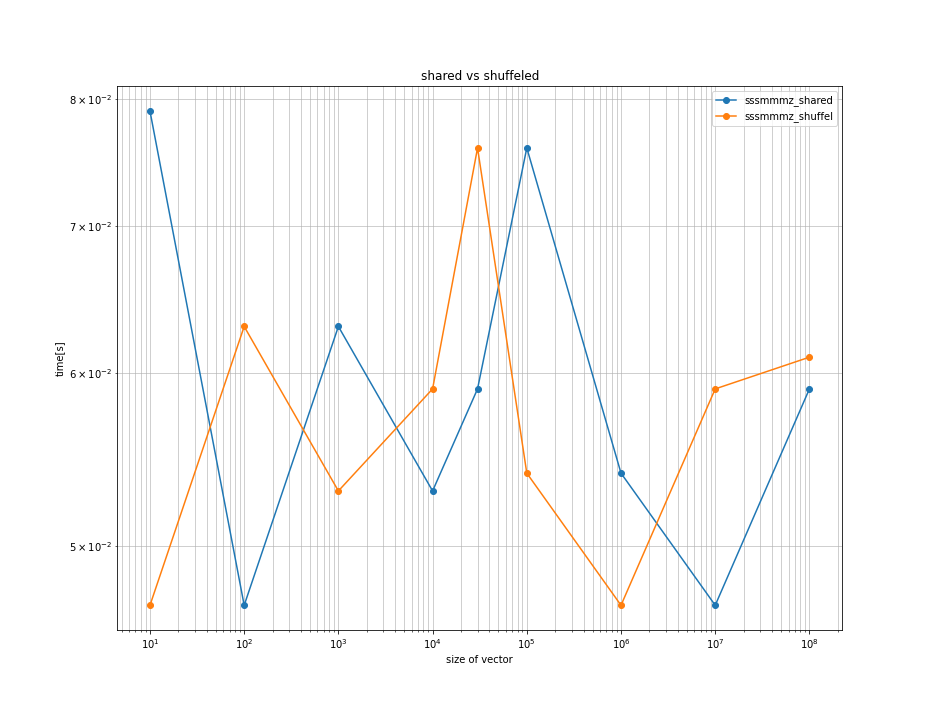
\includegraphics[width=\textwidth]{Bilder/shared_vs_shuffeled}
	\end{minipage}
	\begin{minipage}[t]{0.49\textwidth}
	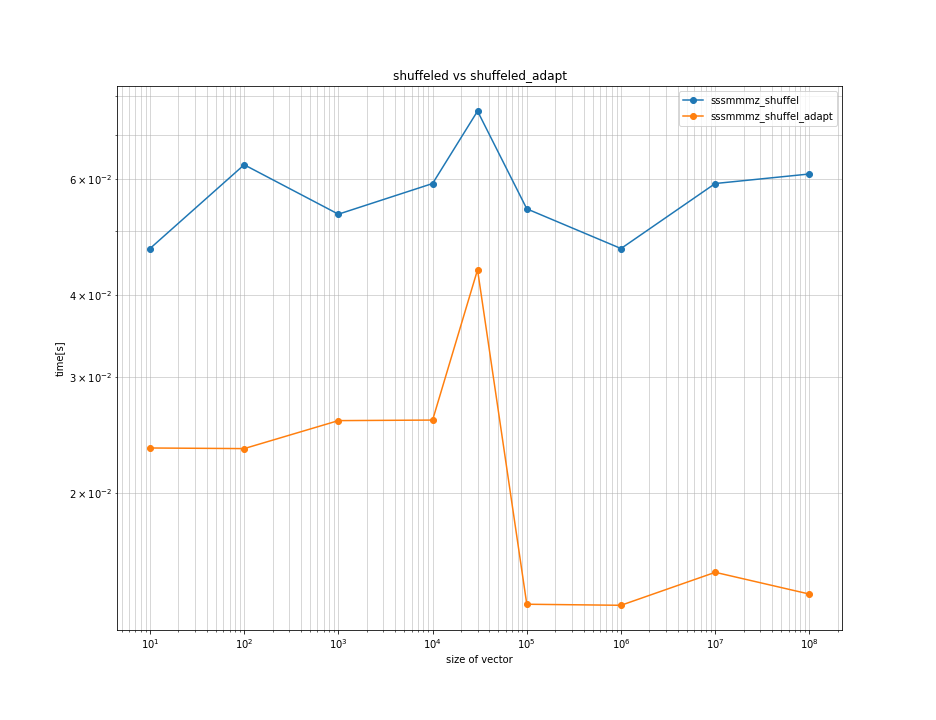
\includegraphics[width=\textwidth]{Bilder/shuffeled_vs_shuffeled_adapt}
	\end{minipage}
	
\end{center}
The "sssmmmz" means the 7 different functions that we have to program into only one kernel. There is a strange oscillation between the two. I tested it also with a multiple number of iterations and always take the mean vaule from that.\\\\
On the left side is the same function plotted but with the worp shuffle instead of the shared memory method. The blue line was tested with a fixed GRID\_SIZE of 128 and a BLOCK\_SIZE of 256. The orange line is the adapt one. It means that the GRID\_SIZE is every step different:
\begin{align*}
GS = \frac{N}{256}
\end{align*}
$GS$ means the GRID\_SIZE. Interesting is that this method is always faster in runtime than the other method.
\begin{center}
	
	\begin{minipage}[t]{0.49\textwidth}
		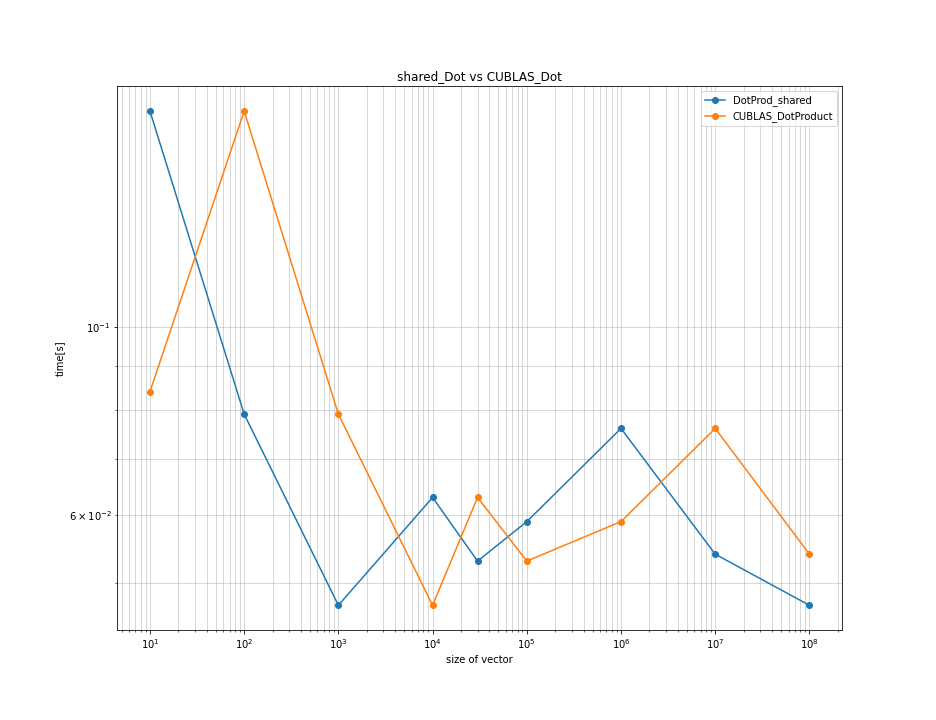
\includegraphics[width=\textwidth]{Bilder/shared_Dot_vs_CUBLAS_Dot}
	\end{minipage}
	
\end{center}
For a small vector size the CUBLAS dot function is slightly slower than the shared one. For higher size vectors is it not clear where the winner is.
\newpage
 \section*{Example 2 Sparse Matrix Times Dense Matrix (3 Points + 1 Bonus)}
 \subsection*{a)}
Use the same function from "poisson.hpp" to populate the matrix $A$. 
  \begin{lstlisting}[language=C++, caption={Kernel for Column-Major}]
__global__ void A_MatMul_Xcm(int N, int K,
int *csr_rowoffsets, int *csr_colindices, double *csr_values,
double *X, double *Y)
{
	int tid = blockIdx.x * blockDim.x + threadIdx.x; 
	if (tid < N)
	{
		int row_start = csr_rowoffsets[tid];
		int row_end = csr_rowoffsets[tid + 1];
		for (int i = row_start; i < row_end; i++) 
		{
			double aij = csr_values[i];
			int row_of_X = csr_colindices[i]*K;
			for (int k = 0; k < K; ++k)
			{
				Y[k + tid*K] += aij * X[row_of_X + k];
			}
		}
	}
}
 \end{lstlisting}
 
\begin{lstlisting}[language=C++, caption={Kernel for Row-Major}]
__global__ void A_MatMul_Xrm(int N, int K,
int *csr_rowoffsets, int *csr_colindices, double *csr_values,
double *X, double *Y)
{
	int tid = blockIdx.x * blockDim.x + threadIdx.x; 
	if (tid < N)
	{
		int row_start = csr_rowoffsets[tid];
		int row_end = csr_rowoffsets[tid + 1];
		
		for (int k = 0; k < K; ++k)
		{
			double sum = 0.0;
			for (int i = row_start; i < row_end; i++) 
			{
				sum += csr_values[i]* X[csr_colindices[i] + k*N];
			}
			Y[k + tid*K] = sum;
		}
	}
}
\end{lstlisting}
 
\begin{lstlisting}[language=C++, caption={Kernel for Standart Matrix Vector}]
__global__ void cuda_csr_matvec_product(int N, int *csr_rowoffsets,
int *csr_colindices, double *csr_values,
double *x, double *y)
{
	for (int i = blockIdx.x * blockDim.x + threadIdx.x; i < N; 
	i += blockDim.x * gridDim.x) 
	{
		double sum = 0;
		for (int k = csr_rowoffsets[i]; k < csr_rowoffsets[i + 1]; k++) 
		{
			sum += csr_values[k] * x[csr_colindices[k]];
		}
		y[i] = sum;
	}
}
\end{lstlisting}

\subsection*{b) results with different N and K}
\begin{center}
	
	\begin{minipage}[t]{0.49\textwidth}
		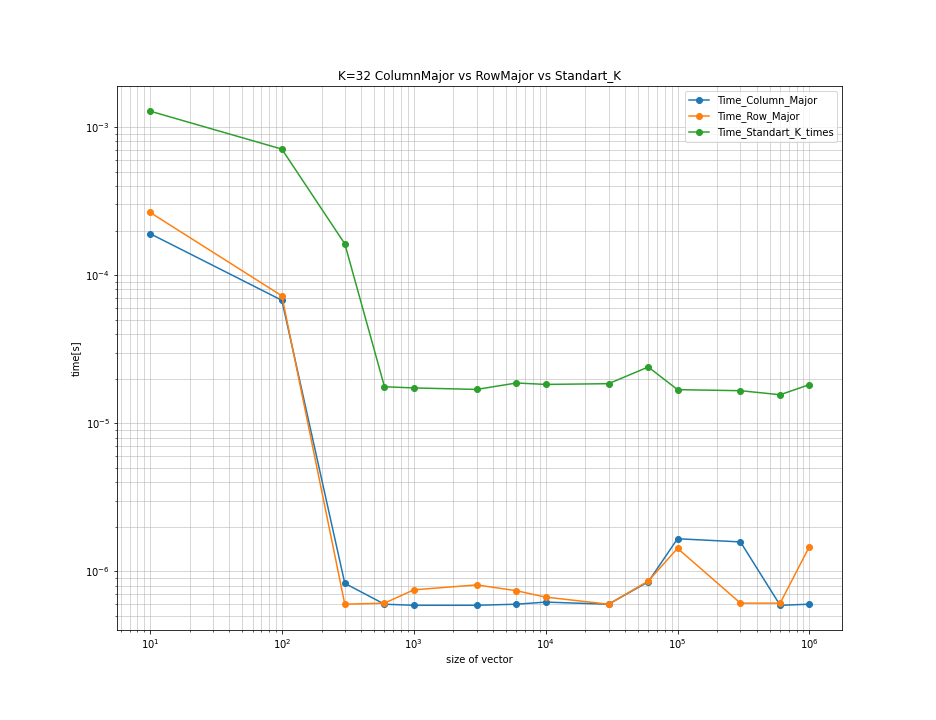
\includegraphics[width=\textwidth]{Bilder/K=32_ColumnMajor_vs_RowMajor_vs_Standart_K.png}
	\end{minipage}
	\begin{minipage}[t]{0.49\textwidth}
		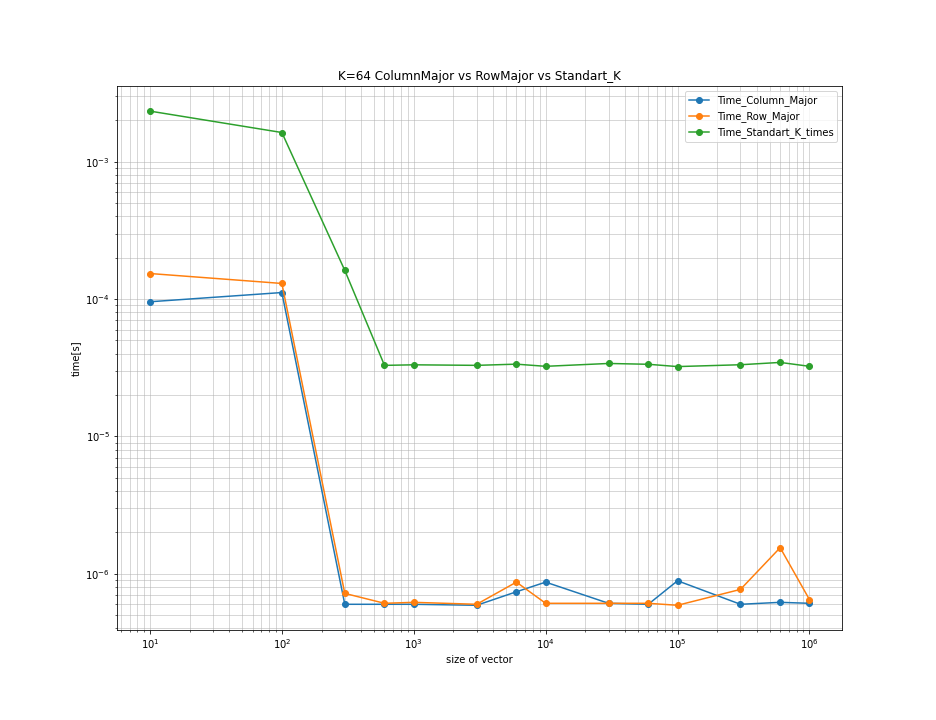
\includegraphics[width=\textwidth]{Bilder/K=64_ColumnMajor_vs_RowMajor_vs_Standart_K.png}
	\end{minipage}
	
\end{center}

\begin{center}
	
	\begin{minipage}[t]{0.49\textwidth}
		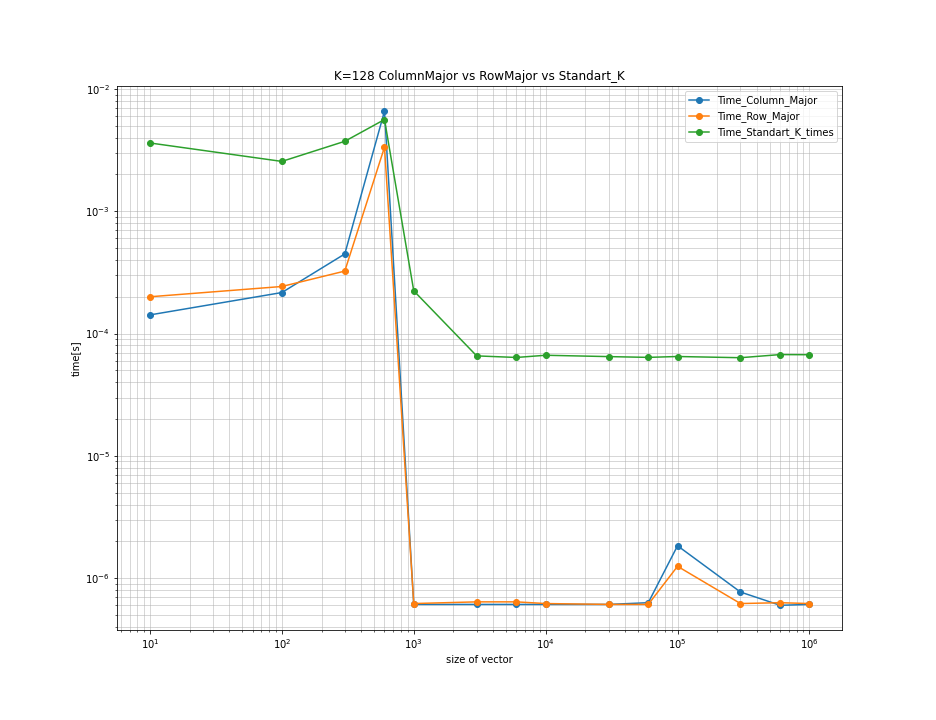
\includegraphics[width=\textwidth]{Bilder/K=128_ColumnMajor_vs_RowMajor_vs_Standart_K.png}
	\end{minipage}
	\begin{minipage}[t]{0.49\textwidth}
		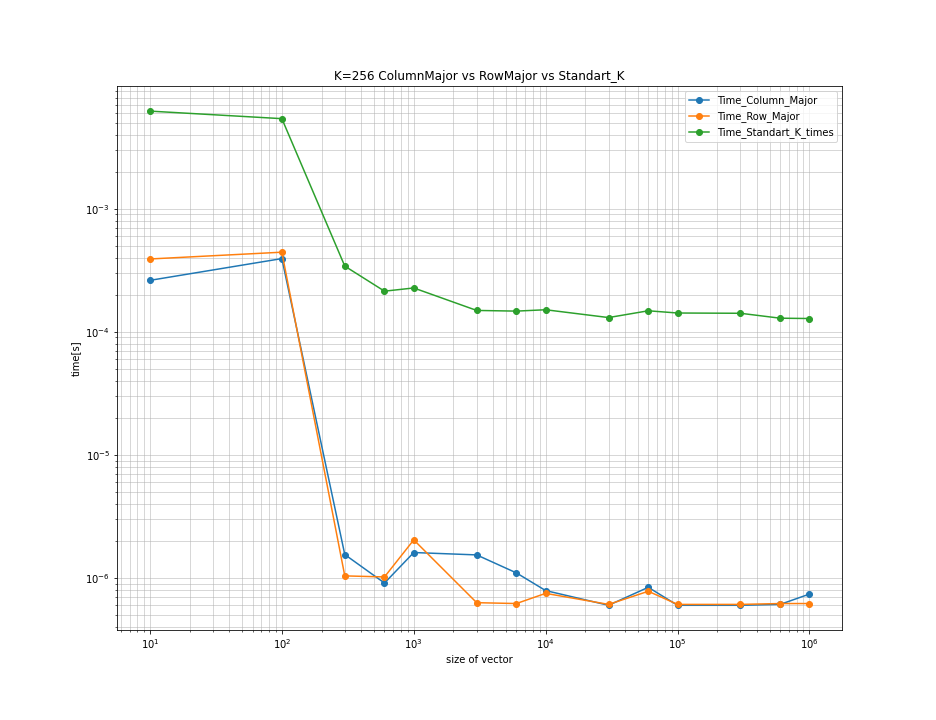
\includegraphics[width=\textwidth]{Bilder/K=256_ColumnMajor_vs_RowMajor_vs_Standart_K.png}
	\end{minipage}
	
\end{center}
\noindent
For increasing number of $K$ the runtimes at a certain point $N = 600$ does not change much. For relatively small numbers of $N$ the runtime is always larger than for large numbers of $N$. I expected the opposite case. For changing number of $K$ the offset between the runtimes at about $N = 1000$ does not change much. There is no difference between the column-major and row-major for different number of $N$ (rows) and number of $K$. The green line is always slower in time as the other two lines.\\\\
\begin{center}
	
	\begin{minipage}[t]{0.49\textwidth}
		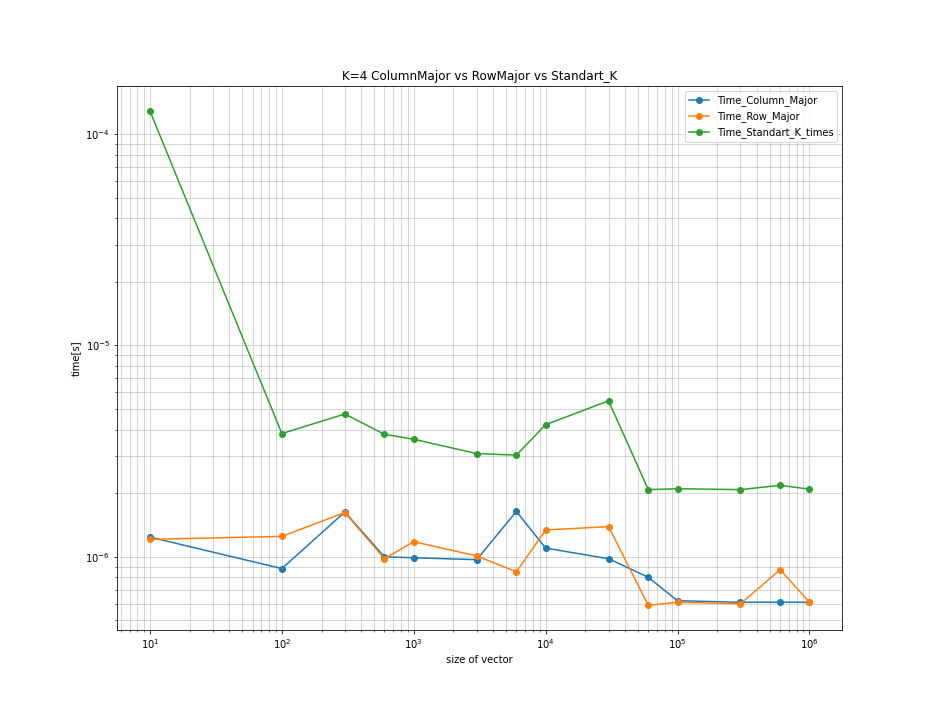
\includegraphics[width=\textwidth]{Bilder/K=4_ColumnMajor_vs_RowMajor_vs_Standart_K.png}
	\end{minipage}
	\begin{minipage}[t]{0.49\textwidth}
		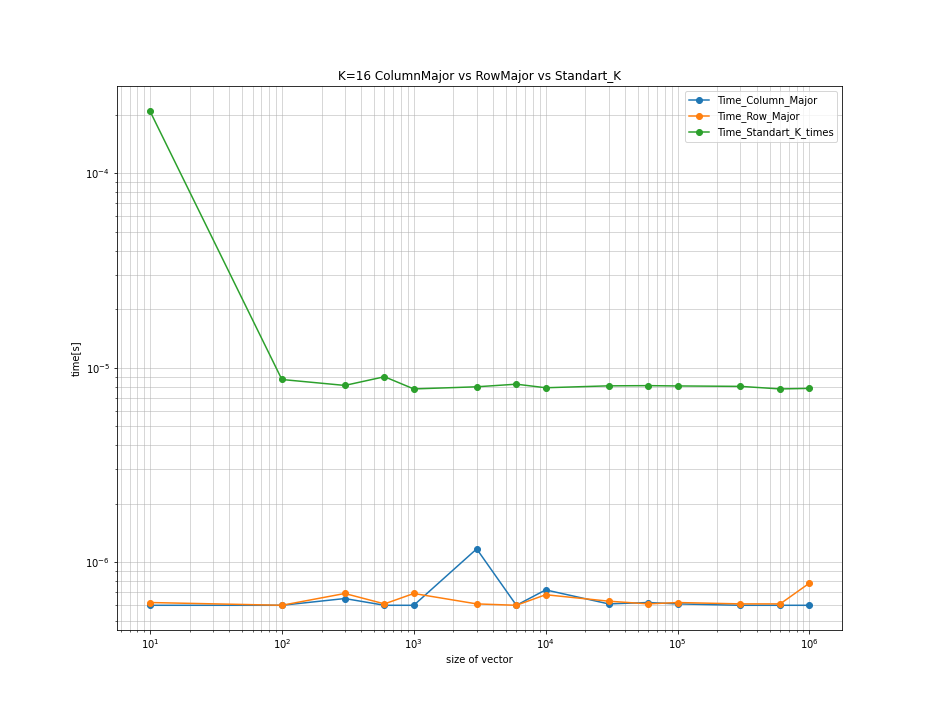
\includegraphics[width=\textwidth]{Bilder/K=8_ColumnMajor_vs_RowMajor_vs_Standart_K.png}
	\end{minipage}
	
\end{center}

\begin{center}
	
	\begin{minipage}[t]{0.49\textwidth}
		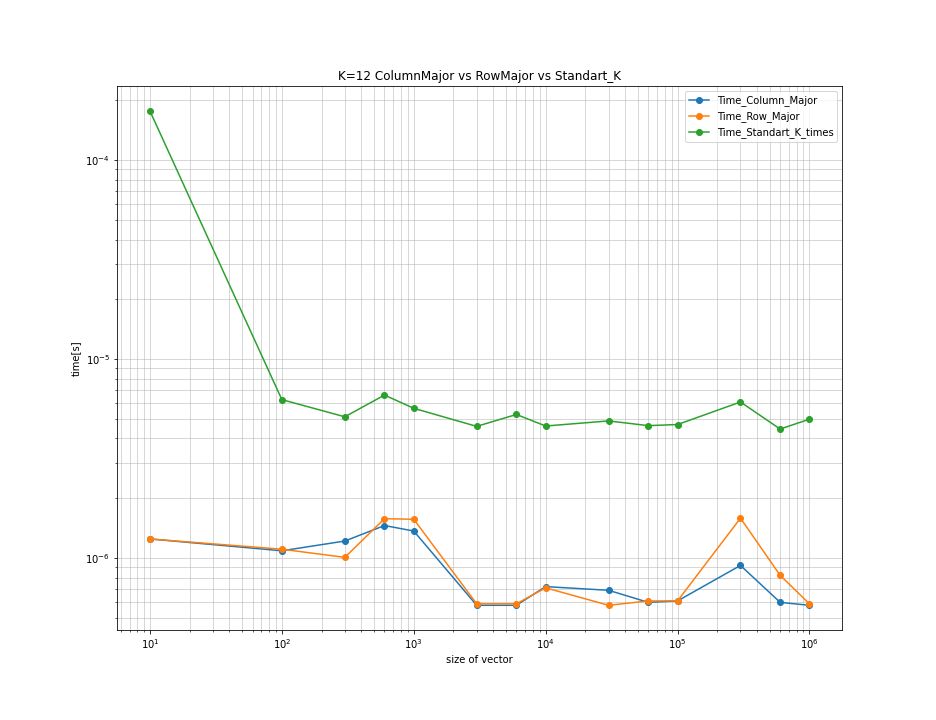
\includegraphics[width=\textwidth]{Bilder/K=12_ColumnMajor_vs_RowMajor_vs_Standart_K.png}
	\end{minipage}
	\begin{minipage}[t]{0.49\textwidth}
		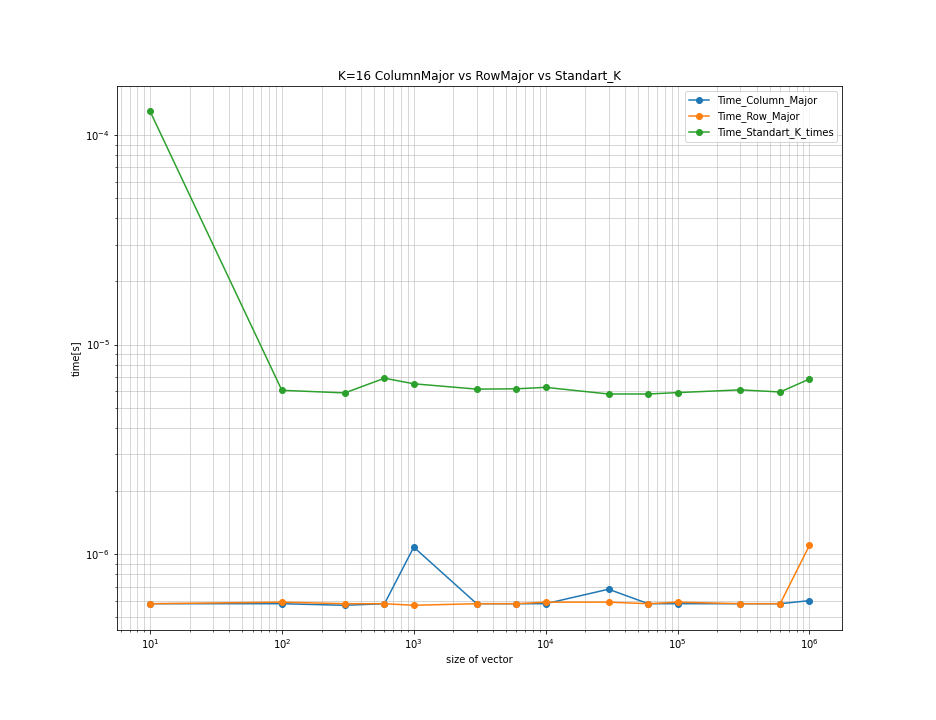
\includegraphics[width=\textwidth]{Bilder/K=16_ColumnMajor_vs_RowMajor_vs_Standart_K.png}
	\end{minipage}
	
\end{center}
First I tested it with low number of $K, \,\,\, K = \{4,8,12,16\}$. But there are basically no differences between the 4 graphs. I expect the runtime grows with the size $N$ of the vector. Or that the row-major method is faster than the column-major method. Because C os more a row-major language instead of for example Fortran.
\end{document}